\documentclass{article}
\usepackage{amsmath}
\usepackage{graphicx} % Required for inserting images

\title{Practice Text Styling}
\author{Md. Roman Nihal}
\date{March 2024}

\begin{document}
\maketitle

\section{Introduction}
Hello \textbf{world}.
I am \textit{Md Roman Nihal.}
My ID is \underline{211902003}
\begin{equation}\label{lim}
    a-b
\end{equation}
\begin{equation}
    a+b
\end{equation}

Equation \ref{lim}was dx

\begin{equation}
    a+b=5+7 %\\
    =12
\end{equation}

\begin{align}
    a+b&=5+7\\
    &=12
\end{align}

\begin{equation}
\begin{split}
    a+b&=5+7\\
    &=12 
\end{split}
\end{equation}

\begin{equation}
    a+b+c+x+y+z=5+4+3+8+121323423+12341324asdaf+dajwjkwja+dffd224asjasd
\end{equation}

\begin{multline}
    a+b+c+x+y+z=5+4+3+8+121323423+12341324asdaf\\+dajwjkwja+dffd224asjasd
\end{multline}

\section{Table}

\newpage

\begin{table}
\caption{Huuha}
\label{er}
\begin{center}
\begin{tabular}{|c|r|}
\hline
     1&2 \\\hline
     322&4423434  \\\hline
\end{tabular} 
\end{center}
\end{table}

the table \ref{er}

\begin{figure}
    \centering
    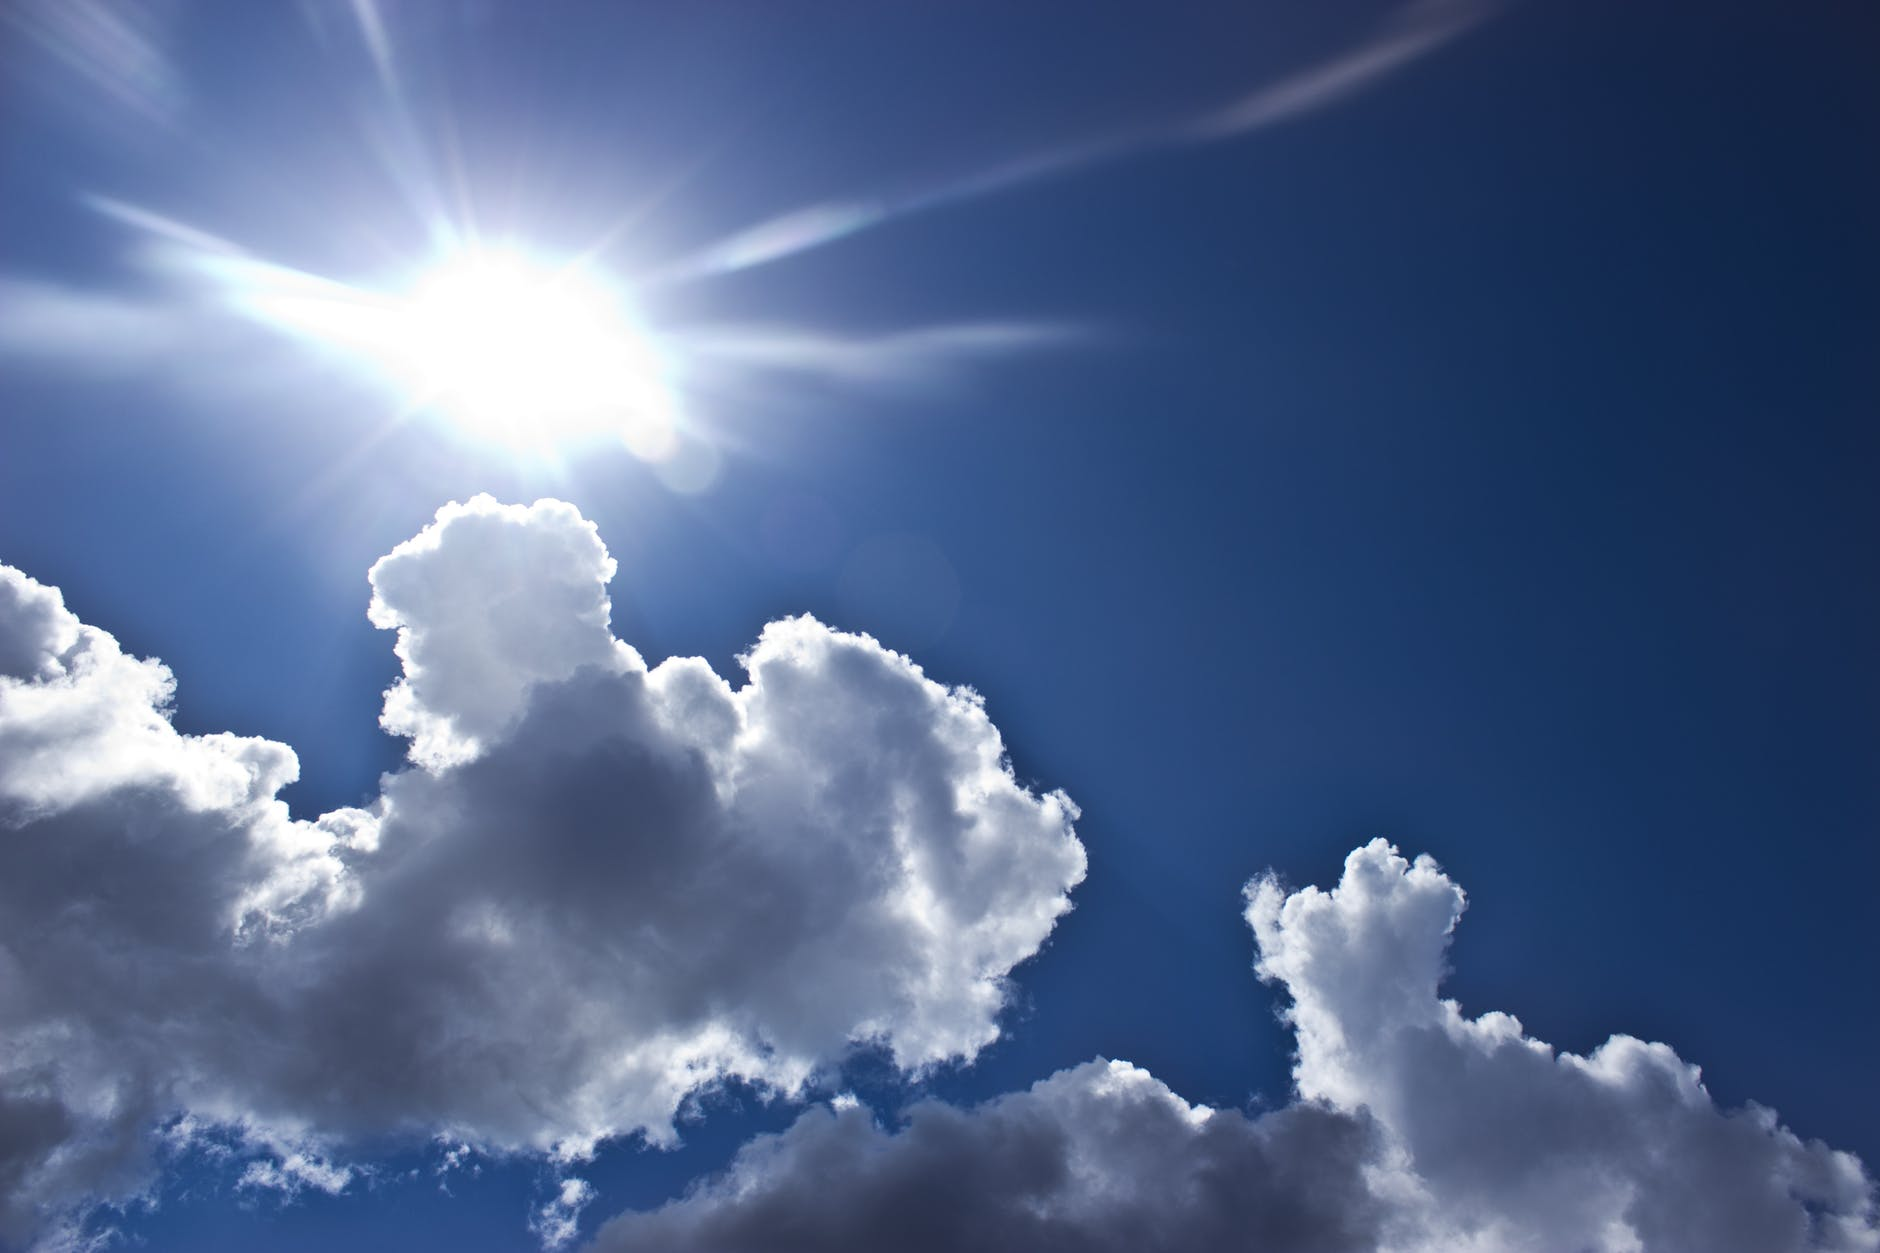
\includegraphics[width=\textwidth]{w.jpeg}
    \caption{sky}
    \label{w}
\end{figure}

the image \ref{w}
\end{document}
